\section{Introduction}
Fluid dynamics is today a cornerstone to several fields of study, including ærospace engineering and meteorology.
Real world fluid behaviour is intricate and complex. Therefore, to gain insights into the governing principles of
fluid flow, simplified and idealized models are used. This essay investigates the application of vector calculus
to model and analyse steady, inviscid, and incompressible fluid flow in two-dimensional spaces around a circular
obstacle. These idealizations allow for the derivation of some of fluid dynamic's key mathematical formulæ and
provides a foundation for understanding less idealized fluids.

This essay will address the question: "\researchquestion" Through the derivation of the velocity potential and
vector field, this essay aims to demonstrate how fundamental laws of fluid motion can be expressed and used through
vector calculus.

% Aim & scope
\subsection{Aim \& scope}
The scope of this essay will be limited to the theoretical modelling of fluid flow in a two-dimensional space
as a vector field under idealized conditions forming steady, inviscid and incompressible fluid flow through the 
derivation of the velocity-potential. The analysis will be centred on the application of vector calculus to derive
fundamental formulæ and describe fluid behaviour around a stationary circular obstacle. Consequently, this essay
will not touch on viscous effects, turbulent flow or three-dimensional analysis, nor will it involve any experimental 
validation. The focus is on the mathematical derivation and analysis of the idealized model.

% Background
\subsection{Background}
\subsubsection{Glossary}
\begin{defn} % steady flow
    \definedterm{Steady flow} refers to flow in which the velocity at every point does not change over time \cite{CRACIUNOIU2001559}.
\end{defn}
\begin{defn} % inviscid flow
    \definedterm{Inviscid flow} is the flow of a fluid with 0 viscosity \cite{ANDERSON20031}.
\end{defn}
\begin{defn} % incompressible fluid
    An \definedterm{incompressible fluid} is a fluid whose density at every point does not change over time \cite{AHMED2019331}. Consequently, this gives rise to the key identity $\div\fatf=0$.
\end{defn}
\begin{defn} % vector field
    A \definedterm{vector field} is a function mapping points in space to vector quantities \cite{BREZINSKI20063}. In the case of fluid dynamics, vector fields often model quantities like fluid velocity.

	\begin{figure*}[!ht]
		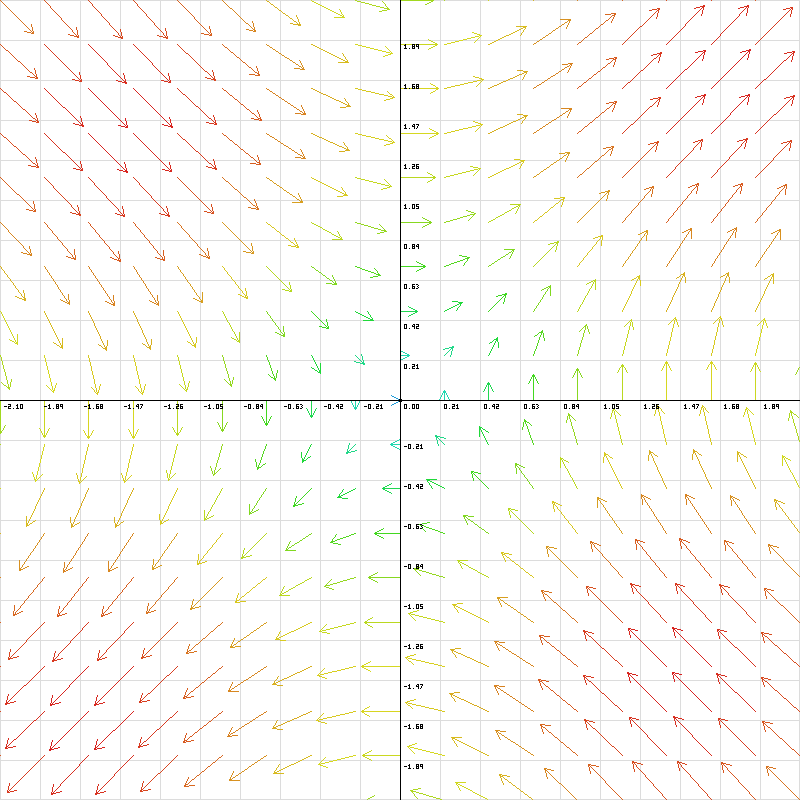
\includegraphics[scale=0.45]{sin.png}
		\centering
		\caption{Vector field plotted for the function $f(x,y)=\begin{pmatrix}
			\sin y\\\sin x
		\end{pmatrix}$}
	\end{figure*}
\end{defn}
\begin{defn} % velocity potential
	The \definedterm{velocity potential} $\phi$ is a scalar quantity whose gradient is the velocity vector field of some fluid, mathematically $\mathbf{V}=\nabla\phi$. The quantity is defined for irrotational flow which is a property of the idealizations made in this essay\referto{theorem:kelvin}.
\end{defn}

\subsubsection{Notation}
In this paper, the gradient, divergence and curl operators will be denoted using their explicit $\nabla$ forms as follows:
$$\begin{matrix}
	\mathrm{grad}\ \fatf&\equiv&\grad{\fatf}\\
	\mathrm{div}\ \fatf&\equiv&\divergence\fatf\\
	\mathrm{curl}\ \fatf&\equiv&\curl\fatf
\end{matrix}$$
The directional vector will also be denoted using $\nabla$ as $\nabla_{\vec{v}}\fatf$.

For the purposes of clarity, vectors in cartesian systems will be denoted $\begin{pmatrix}x\\y\end{pmatrix}$ whilst vectors in polar systems will be denoted as $\langle r,\theta\rangle$

To ensure point-uniqueness within polar systems, all polar coordinates are restricted such as $r\geq0,\,\theta\in[0,2\pi)$.